\newprob{1715830312}
{
    在一個實驗中,將電熱水器內2 kg \oc{20}的水加熱就20分鐘。水被加熱至\oc{100}沸騰後只餘下1.7 kg的水。電熱水器功率的估算值是多少?
    \par 己知:水的比熱容量=\shc{4200},水的汽化比潛熱=\slh{2.26e6}
    % \par In an experiment, 2kg of water at \oc{20} is heated inside a boiler for 20 minutes. Water is boiled to \oc{100} and 1.7kg of water remains after boiling. What is the estimated power of the boiler?
    % \par Given: Specific heat capacity of water = \shc{4200}, specific latent heat of vaporization of water = \slh{2.26e6}.
    \begin{figure}[h]
        \centering
        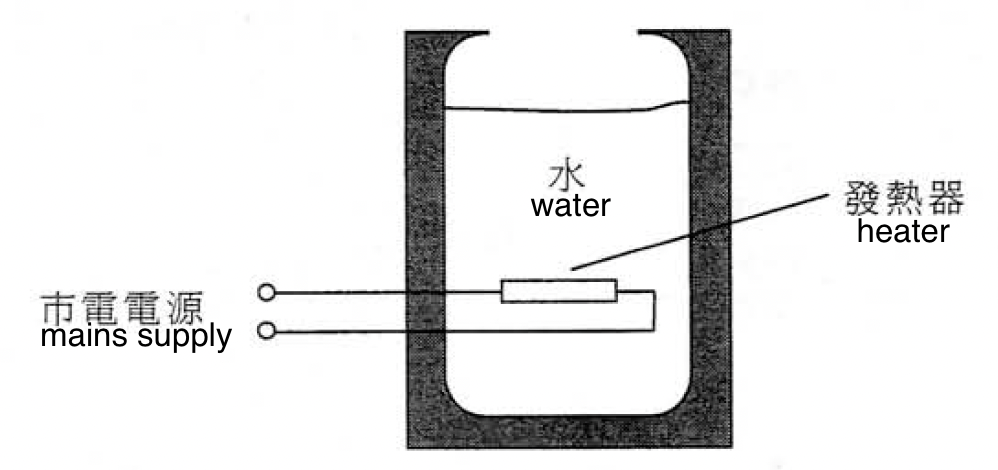
\includegraphics[width=0.35\linewidth]{assets/Screenshot 2023-09-13 at 10.23.39 PM.png}
    \end{figure}
    \begin{choices}
        \choice 565 W
        \choice 649 W
        \CorrectChoice 1125 W
        \choice 3762 W
    \end{choices}
}{}

\newprob{1715831569}
{
    以下數據顯示了四種質量相同的物質 P、Q、R 和 S 的熱性質:
    % \par The following data shows the thermal properties of four substances of the same mass P, Q, R and S:\flushhere
    \begin{table}[!ht]
        \centering
        \begin{tabular}{|c|c|c|c|c|}
            \hline
            物質Substance                                                   & P          & Q          & R          & S           \\ \hline
            熔點Melting point                                               & 40K        & 98K        & 114K       & 270K        \\ \hline
            沸點Boiling point                                               & 280K       & 880K       & 180K       & 370K        \\ \hline
            平均比熱容量 Average specific heat capacity \unit{J.kg^{-1}.K^{-1}} & 800        & 1200       & 226        & 40          \\ \hline
            熔解比潛熱 Specific latent heat of fusion \unit{J.kg^{-1}}         & \num{2e4}  & \num{11e4} & \num{5e4}  & \num{33e4}  \\ \hline
            汽化比潛熱 Specific latent heat of vaporization \unit{J.kg^{-1}}   & \num{30e4} & \num{34e4} & \num{40e4} & \num{230e4} \\ \hline
        \end{tabular}
    \end{table}
    當温度從250 K提升至40 K,哪個物質會吸收最高的熱?
    % When the temperature of each substance is increased from 250K to 400K, which one will absorb the most heat?
    \begin{choices}
        \choice P
        \choice Q
        \choice R
        \CorrectChoice S
    \end{choices}
}{}

\newprob{1715831636}
{
    以下哪項是正確的?
    % Which of the following descriptions is correct?
    \begin{choices}
        \choice 當 \oc{25}的水加熱至 \oc{50},水分子的動能和勢能上升。
        % \par When water at \oc{25} is heated to \oc{50}, both the kinetic energy and potential energy of the water molecules increase.
        \choice 當 \oc{25}的水加熱至 \oc{50},水分子的勢能上升。
        % \par When water at \oc{25} is heated to \oc{50}, only the potenial energy of water mmolecule increases.
        \choice 當水在 \oc{100}沸騰且轉化成蒸氣時,水分子的動能上升。
        % \par When water boils at \oc{100} and turns into steam, the kinetic energy of water molecules increases.
        \CorrectChoice 當水在 \oc{100}沸騰且轉化成蒸氣時,水分子的勢能上升。
        % \par When water boils at \oc{100} and turns into steam, the potential energy of the water molecules increases.
    \end{choices}
}{}

\newprob{1715831657}
{
    以下哪項是正確的?
    % Which of the following statements is correct?
    \begin{enumerate}[label=\sd]
        \item 物態轉變時,物質的溫度保持不變。
              %   \par The temperature of a substance remains unchanged when it changes state.
        \item 水凝固的溫度等於水的熔點。
              %   \par The freezing point of water is equal to the melting point of ice.
        \item 蒸汽的溫度比定大於水的溫度。
              %   \par The temperature of steam is always higher than that of water.
    \end{enumerate}
    \begin{choices}
        \CorrectChoice 只有(1)和(2)
        \choice 只有(1)和(3)
        \choice 只有(2)和(3)
        \choice (1), (2) 和 (3)
    \end{choices}
}{}

\newprob{1715831687}
{
    一個熱容量極小的電熱水壺用來煮水。它將水從\oc{25}加熱到\oc{100},用了6分鐘的時間。如果恆溫器失靈,並且忘記關掉電源,估計從沸騰的一刻起,全部水被汽化所需的時間。(忽略向周圍環境散失的熱量。)
    己知:水的比熱容量 = \shc{4200},水的汽化比潛熱 = \slh{2.26e6}
    % \par An electric kettle of negligible heat capacity is used to boil some water. It heats up the water from \oc{25} to its boiling point \oc{100} in 6 min. If the thermostat fails and one forgets to turn off the power supply, estimate how long it will take from boiling to vaporizing the water completely. (Neglect heat lost to the surroundings.)
    % Given: specific heat capacity of water= \shc{4200}, specific latent heat of vaporization of water = \slh{2.26e6}.
    \begin{choices}
        \choice 8分鐘
        \CorrectChoice 43分鐘
        \choice 55分鐘
        \choice 無從得知,因為水的質量沒有提供
    \end{choices}
}{}

\newprob{1715831714}
{
    在雪融化的時候,人們通常感覺比正在下雪的時候更冷。這主要是因為
    % \par During the time when snow melts, people usually feel colder than the time when snow falls. This is mainly because

    \begin{choices}
        \choice 人的感覺是不可靠的。
        % \par Human sensation is not reliable.
        \choice 雪融化的溫度低於\oc{0}。
        % \par Snow melts at a temperature below \oc{0}.
        \choice 下雪時釋放了內能。
        % \par Internal energy is released by falling snow.
        \CorrectChoice 當雪融化時,它會從周圍吸收大量的潛熱。
        % \par When snow melts, it absorbs a lot of latent heat from surroundings.
    \end{choices}
}{}

\newprob{1715831734}
{
    一個電熱水壺中的水正在穩定沸騰。如果現在增加水壺的功率,以下哪些說法是正確的?
    % \par Water is boiling steadily in an electric kettle. If the power of the kettle is now increased, which of the following statements is/are correct?
    \begin{enumerate}[label=\sd]
        \item 水的溫度上升。
              %   \par The temperature of the water increases.
        \item 水的內能上升。
              %   \par The internal energy of the water increases.
        \item 水以更快的速率汽化。
              %   \par Water vaporizes at a greater rate.
    \end{enumerate}
    \begin{choices}
        \choice 只有(1) \tab (1) only
        \choice 只有(2) \tab (2) only
        \CorrectChoice 只有(3) \tab (3) only
        \choice (1), (2) 和 (3)\tab (1), (2) and (3)
    \end{choices}
}{}

\newprob{1715831759}
{
    一位農民為了在寒冷的冬天保持馬廄的溫暖,在馬廄裡放置了840 kg,\oc{10},在太陽下加熱的桶裝水。晚上,水從 \oc{10}冷卻到 \oc{0}並完全凝結成冰。在這個過程中,釋放了大量的熱量。如果要產生相同的熱量,一個2kW的暖氣爐需要運行多少小時(h)?(水的比熱容量= \shc{4200},冰的熔解比潛熱= \slh{3.34e5})
    % \par To help keeping his stable warm on cold winter days, a farmer stores 840kg of solar-heated water at \oc{10} in barrels placed inside the stable. At night the water cools from \oc{10} and completely freezes to become ice at \oc{0}. During this process, a large amount of heat is released. For how many hours (h) would a 2 kW space heater be operated to produce the same amount of heat?
    % (specific heat capacity of water= \shc{4200}, specific latent heat of fusion of ice = \slh{3.34e5})
    \begin{choices}
        \choice 24h
        \choice 38.9h
        \CorrectChoice 43.9h
        \choice 269h
    \end{choices}
}{}